\documentclass[12pt, specialist, subf, substylefile = spbu.rtx]{disser}
\usepackage[a4paper, includefoot,
            left=3cm, right=1.5cm,
            top=2cm, bottom=2cm,
            headsep=1cm, footskip=1cm]{geometry}
\usepackage[utf8]{inputenc}
\usepackage[T1, T2A]{fontenc}
\usepackage[english, russian]{babel}
\usepackage{moreverb}
\usepackage{array}
\usepackage{hyperref}
\usepackage{amsthm}
\setcounter{tocdepth}{2}
\graphicspath{{diploma3_fig/}}
\newtheorem{theorem}{Теорема}
\newtheorem{definition}{Определение}
\newtheorem{algo}{Алгоритм}
\newcommand{\Expect}{\mathsf{E}}
\newcommand{\CVaR}{\mathsf{CVaR}}
\newcommand{\Var}{\mathsf{Var}}
\DeclareGraphicsExtensions{.pdf}
\DeclareMathOperator*{\toplim}{\overline\lim}
\DeclareMathOperator*{\botlim}{\underline\lim}
\DeclareMathOperator*{\tou}{\longrightarrow}
\newcommand{\MDA}{\mathsf{MDA}}
\begin{document}

% Титульный лист


\institution{%
    Санкт-Петербургский государственный университет \\
    Прикладная математика и информатика \\
    Статистическое моделирование
}
\title{Отчет о научно-исследовательской работе}
\topic{\normalfont\scshape %
Доверительное оценивание параметров предельных распределений статистик экстремальных значений}
\author{Старков Артём Константинович}

\sa {М.\,С.~Ермаков}
\sastatus{д.\,ф.-м.\,н., профессор}


\city{Санкт-Петербург}
\date{\number\year}

\maketitle

\tableofcontents


\intro
%% Введение

В вопросах оценивания вероятностей больших уклонений весьма важную роль играет вопрос о распределении максимумов. Например, пусть дана последовательность независимых случайных величин $(X_i)_{i=1}^n$. Тогда $M_n$ --- их выборочный максимум: 
$$
M_n=\max(X_1, ..., X_n).
$$

Одним из результатов изучения распределения $M_n$ является теория предельных распределений. Важнейший результат этой теории заключен в теореме, представленной ниже~\cite[стр.~132]{Embrechts}.
\begin{theorem}[Фишера-Типпета-Гнеденко]\label{th:ftg}
Пусть $(X_i)_{i=1}^n$ --- последовательность независимых случайных величин, $M_n$ --- их выборочный максимум $M_n=\max(X_1, ..., X_n).$ Если существуют такие $c_n>0, d_n \in \mathbb{R}$ и некоторая плотность распределения $H$, что выполняется
$$
\frac{(M_n-d_n)}{c_n} \tou^p H,
$$
тогда $H$ принадлежит одному из семейств предельных распределений:

\begin{tabular}{lll}
\text{Фреше:} 
	& $ \Phi_\alpha(x)=e^{-x^{-\alpha}}, $ 
	& $ x>0, \alpha>0; $ \\
\text{Вейбулл:} 
	& $ \Psi_\alpha(x)=e^{-(-x)^\alpha}, $ 
	& $ x \le 0, \alpha>0; $ \\
\text{Гумбель:}
	& $ \Lambda(x)=e^{-e^{-x}}, $ 
	& $ x \in \mathbb{R}. $ \\
\end{tabular}
\end{theorem}

Очевидно, что вид предельного распределения напрямую зависит от исходного распределения $X_i$. Будем говорить, что если некоторая последовательность $(X_i)_{i=1}^n$ с функцией распределения $F(x)$ имеет предельное распределение $H$, то она принадлежит его области максимального притяжения (maximum domain attraction), и записывать:
$$
F \in \MDA(H).
$$

В книге Гумбеля~\cite[стр.~194]{Gumbel} детально изложен вывод предельных распределений из теоремы~\ref{th:ftg}, данный Фишером и Типпетом. Там же продемонстрирован общий вид распределений, предложенный Дженкинсоном:
\begin{equation}\label{eq:phi}
\Phi(x)=\exp\left[-\left(1-\frac{x}{a}\right)^{\frac{1}{k}}\right], ak>0.
\end{equation}

В данной работе рассматривается распределение Фреше. Оно соответствует семействам распределений Парето, Коши, Булла и др. (для случая $k<0$ из~\eqref{eq:phi}).

Распределение Фреше имеет параметры shape $\alpha$, scale $s$ и location $m$; $\alpha>0, s>0, x>m$:
$$ F(x)=e^{-(\frac{x-m}{s})^{-\alpha}}, $$
$$ p(x)=\frac{\alpha}{s} \left(\frac{x-m}{s}\right)^{-1-\alpha} e^{-(\frac{x-m}{s})^{-\alpha}}.$$

Для $\MDA(\Phi_\alpha)$ существует следующая теорема~\cite[стр.~142]{Embrechts}:
\begin{theorem}\label{th:freclim}
Функция распределения $F(x)$ принадлежит области максимального притяжения распределения Фреше $F \in \MDA(\Phi_\alpha)$ для $\alpha > 0$, если и только если $\bar{F}(x)=x^{-\alpha}L(x),$ для некоторой медленно меняющейся функции $L$, где $\bar{F}(x)=1-F(x)$ --- распределение хвоста $F(x)$.
\end{theorem}
На основании этого факта Хиллом~\cite{Hill} была получена оценка для $\alpha$, совпадающая с оценкой максимального правдоподобия:
\begin{equation}\label{eq:hillEstLower}
\hat{\alpha}_H=\left(\frac{1}{k} \sum\limits_{i=1}^k \ln X_{i:n}-\ln X_{k:n} \right)^{-1},
\end{equation}
где $k=k(n) \to \infty$. Это оценка т.н. <<нижнего хвоста>> (\textit{lower tail estimate}), в той же статье делается оценка и <<верхнего хвоста>> (\textit{upper tail estimate}), т. е. для распределения хвоста на интервале $[\beta, 1)$. Она идентична~\eqref{eq:hillEstLower} и делается путем замены $X=Y^{-1}$; соответственно с учетом смены направления упорядочивания вариационного ряда получаем 
$$
Y_{i:n}=X_{n-i+1:n},
$$
\begin{equation}\label{eq:hillEst}
\left(\frac{1}{n-m+1} \sum\limits_{i=m}^n \ln X_{i:n}-\ln X_{m:n} \right)^{-1},
\end{equation}
где $m=n-k+1 : m=[\beta n]$.

Для многих прикладных задач параметр $\alpha$ имеет большое значение. Например, при $\alpha<2$ дисперсия бесконечна: $\Expect X^2=\infty.$ Этот случай часто наблюдается на практике, и его нужно отслеживать при моделировании. В связи с этим возникает задача определения качества полученной оценки. Так как оценка строится в условиях $k=k(n) \to \infty$, то любая попытка определения качества оценки затруднительна ввиду необходимости получения большого количества реализаций $n \to \infty$ при том, что действительно полезных из них будет относительно немного (в зависимости от параметра $\beta$). В решении этой проблемы в задачах статистического моделирования может помочь асимптотическая эффективность метода существенной выборки.

%% Метод существенной выборки
\section{Метод существенной выборки}

Пусть поставлена задача вычисления следующей вероятности:
\begin{equation}\label{eq:sv_pt}
\omega=P(T(\hat{P}_n)-T(P_0) \in b_n\Omega),
\end{equation}
где $P_0$ -- теоретическое распределение; $\hat{P}_n$ -- эмпирическая функция распределения; $T(P)$ -- некоторый функционал. Согласно методу, необходимо выбрать меру $Q_n$ такую, что $Q_n \ll P_0$. Затем моделируются $k$ независимых выборок с распределением $Q_n$
$$
Y_1^{(i)}, Y_2^{(i)}, ... , Y_n^{(i)}, 1 \le i \le k.
$$

Оценка вероятности:
\begin{equation}\label{eq:sv_sd}
\hat{\omega}_n=\frac{1}{k} \sum\limits_{i=1}^{k}
\chi \big(T(\hat{Q}^{(i)}_n)-T(P_0) > b_n\big)
\prod\limits_{j=1}^{n} q_n^{-1}(Y_j^{(i)}),
\end{equation}
где $\hat{Q}^{(i)}_n$ -- эмпирическое распределение выборки $Y^{(i)}_j$, $q_n=\frac{dQ_n}{dP_0}$.

Введем величину
$$
U_n=\Expect_{Q_n} 
\left[   
\chi \big(T(\hat{Q}^{(1)}_n)-T(P) > b_n\big)
\prod\limits_{j=1}^{n} q_n^{-2}(Y_j^{(1)})
\right],
$$
тогда дисперсия оценки~\eqref{eq:sv_sd} имеет вид
$$
V(Q_n)=\Var[\hat\omega_n]=U_n-\omega_n^2,
$$
где $\omega_n$ -- математическое ожидание~\eqref{eq:sv_sd}. Потому естественно рассмотреть асимптотическую эффективность процедуры существенной выборки. Будем определять ее в терминах теории вероятности больших уклонений. В силу неотрицательности дисперсии ясно, что
$$
U_n \le \omega_n^2.
$$

\begin{definition}
Процедура называется асимптотически эффективной (в смысле логарифмической асимптотики), если 
$$
\overline{\lim\limits_{n \to \infty}} \frac{\log U_n}{2 \log \omega_n} = 1.
$$
\end{definition}

\begin{definition}
Процедура называется эффективной, если 
$$
\overline{\lim\limits_{n \to \infty}} \frac{U_n}{2 \omega_n} = 1.
$$
\end{definition}

Так как задачей является оценка малых вероятностей, их математические ожидания и дисперсии также будут малыми величинами. Тогда даже малые ошибки в вычислениях могут привести к значительным ошибкам в значении эффективности или даже невозможности ее вычислить. На асимптотическую эффективность малые ошибки влияют незначительно; поэтому для определения качества процедуры будет использоваться асимптотическая эффективность.

Основной трудностью при использовании метода существенной выборки является выбор меры $Q_n$ при условии достижения процедурой асимптотической эффективности.

Предпосылкой для решения задачи о выборе меры $Q_n$ стала работа математика И. В. Санова. Им была исследована задача вычисления вероятности 
\begin{equation}\label{eq:sv_san}
P(\hat{P}_n \in \Omega),
\end{equation}
где $\hat{P}_n$ -- эмпирическая функция распределения, построенная по выборке $X_i \sim P_0, 1 \le i \le n$; $\Omega$ принадлежит пространству мер. Он исследовал асимптотическое поведение вероятности~\eqref{eq:sv_san} и получил следующие результаты:
\begin{equation}\label{eq:sv_san2}
\begin{tabular}{l}
$\toplim\limits_{n \to \infty} \frac{1}{n} \ln P(\hat{P}_n \in \Omega) \le -\inf\limits_{H\in \mathfrak{int}(\Omega)} K(H, P_0),$
\\
$\botlim\limits_{n \to \infty} \frac{1}{n} \ln P(\hat{P}_n \in \Omega) \ge -\inf\limits_{H\in \mathfrak{cl}(\Omega)} K(H, P_0),$
\end{tabular}
\end{equation}
где $\mathfrak{int}(\Omega)$ и $\mathfrak{cl}(\Omega)$ -- соответственно замыкание и внутренность $\Omega$ в специальной топологии со слабой сходимостью, 
\begin{equation}\label{eq:sv_k}
K(H, P_0)=
\begin{cases}
\int \ln \frac{dH}{dP_0}dH, 
	&\text{если $H \ll P_0$;}\\
\infty,	
	&\text{иначе.}
\end{cases}
\end{equation}

На основе этих результатов в дальнейшем была развита теория вероятности больших уклонений, окончательно формализованная С. Р. Варадханом. В рамках этой теории неравенства типа~\eqref{eq:sv_san2} стали называться принципом больших уклонений, а функционалы типа~\eqref{eq:sv_k}
-- функционалами действия. Они являются в некотором смысле мерой близости распределений $H$ и $P_0$, схожей с расстоянием Кульбака-Лейблера.


Рассмотрим задачу~\eqref{eq:sv_pt} в зоне больших уклонений:
$$
P(T(\hat{P}_n)-T(P_0) \in \Omega), \Omega \in \mathbb{R}.
$$
На практике для такой задачи нахождение $H$ часто является неразрешимой задачей. В зоне умеренных уклонений и действия ЦПТ для задачи в виде
\begin{equation}\label{eq:sv_ptum}
P(T(\hat{P}_n)-T(P_0) \in b_n\Omega), \Omega \in \mathbb{R},
\end{equation}
где $nb_n^2 \to \infty, b_n \to \infty$, действует нормальная асимптотика, но для логарифма распределения. Здесь задача нахождения $H$ разрешима для очень широкого класса функционалов $T$.

М. Джонсоном была построена асимптотически эффективная процедура метода существенной выборки в зоне нормальной аппроксимации. В зону умеренных уклонений его результаты были перенесены М. С. Ермаковым в статье~\cite{Ermakov}. В статье рассматривается задача~\eqref{eq:sv_ptum} в случае, когда статистика $T(\hat{P}_n)$ имеет функцию влияния $g$ и верны предположения, рассматриваемые ниже.

Введем следующие множества: 
\begin{enumerate}
\item множество функций $\Phi$ такое, что для любой $f \in \Phi$  $\Expect f(x)=0 $ и
$$
\lim\limits_{n \to \infty} \frac{1}{nb_n^2} \log \big(nP_0(|f(X)|>nb_n)\big)=-\infty;
$$

\item множество $\Lambda_\Phi$ всех мер $Q \in \Lambda$ таких, что для любой $f \in \Phi$
$
\int\limits_{\Omega} |f| dQ < \infty;
$

\item множество $\Lambda_{0\Phi}$ всех зарядов $G=P-R; P, R \in \Lambda$.

\end{enumerate}

Тогда предположим, что $g \in \Phi$ и существует полунорма $N \in \Lambda_{0\Phi}$, такая, что для любого $Q \in \Lambda_\Phi$
$$
|T(Q)-T(P_0)-\int\limits_{\Omega}g dQ| \le 
\omega\big(N(Q-P_0), \int\limits_{\Omega}g dQ, T(Q)-T(P_0) \big)
$$
с функцией $\omega\colon \mathbb{R}^3 \to \mathbb{R}_+$, такой, что
$$
\lim\limits_{t_1, t_2, t_3 \to 0} \frac{\omega(t_1, t_2, t_3)}{t_1+ t_2+t_3} = 0.
$$

М. С. Ермаковым была доказана следующая теорема.
\begin{theorem}\label{th:erm}
В предположениях, изложенных выше, рассмотрим процедуру существенной выборки, основанную на вероятностной мере $Q_n$ с плотностью 
$$
q_{1n}(x)=\lambda_n+b_nh(x)\chi\left(h(x)>-\frac{\delta}{b_n}\right)
$$
или
$$
q_{2n}(x)=c_ne^{b_nh(x)} \chi\left(h(x)<\frac{\delta}{b_n}\right),
$$
где $\lambda_n, c_n$ -- константы нормализации, $\delta \in [0, 1]$ и $\Expect h(x)=0, \Expect|h(x)|<\infty, \Expect h^2(x)< \infty$. Тогда процедура существенной выборки асимптотически эффективна, если $h=\frac{g}{\sigma^2_g}$

\end{theorem}


%% Постановка задачи
\section{Постановка задачи}

Пусть $(X_i)_{i=1}^n$ --- независимые случайные величины с функцией распределения $F \in \MDA(\Phi_\alpha)$. Упорядочим выборку по возрастанию, получим вариационный ряд:
$$
X_{1:n} \le X_{2:n} \le ... \le X_{n:n}.
$$

Хвост распределения $\bar{F}(x)=1-F(x)$ принадлежит семейству предельного распределения Фреше $\Phi_\alpha$, в котором неопределенным остается параметр формы (shape) $\alpha$. Имеем для него оценку Хилла:
\begin{equation}\label{eq:hill_est}
\hat{\alpha}_H=
\left(\frac{1}{n-m+1} \sum\limits_{i=m}^n \ln X_{i:n}-\ln X_{m:n} \right)^{-1},
\end{equation}
где $m=[\beta n]$.


Рассмотрим задачу оценки вероятности уклонения оцененного значения от истинного, представленной в формуле~\eqref{eq:sv_pt}, где в качестве функционала $T(F)$ будет выступать оценка $\hat{\alpha}_H$. Так как сама оценка строится в условиях $m=m(n) \to \infty$, то $\beta \to 1$, и обычные оценки становятся неэффективными. Для решения данной проблемы будет использована асимптотическая эффективность метода существенной выборки.

По теореме \ref{th:erm} будем использовать вероятностную меру $Q_n$ вида
\begin{equation}\label{eq:g_common}
g(x)=p(x)(1+b_nh(x)),
\end{equation}
где $h(x)$ --- функция влияния оцениваемого функционала, $b_n$ -- константа для определения ширины доверительного интервала, 
\begin{equation}\label{eq:bn}
b_n = \pm\frac{N_{(0,1)}^{-1}(\gamma)}{\sqrt{n}\sigma},
\end{equation}
\begin{equation}\label{eq:asymdisp}
\sigma^2(F)= \int_-\infty^\infty \int_-\infty^\infty J(F(x)) J(F(y))\big( F(x \wedge y)-F(x)F(y)\big)
\end{equation}
--- асимптотическая дисперсия функционала $T(F)$.

Определим вид оцениваемого функционала и его функцию влияния.

Для удобства будем оценивать значение $\hat{\alpha}_H^{-1}$; таким образом избавляемся от показателя степени $-1$ в правой части. Обозначим $Y_j=\ln X_j$, тогда $F_y(\ln t)=F(t)$, $F_y$ -- функция распределения $Y$. Получим следующий функционал:
\begin{equation}\label{eq:t_f_y}
T(F_y)=\hat{\alpha}_H^{-1}=\frac{1}{n-m+1} \sum\limits_{i=m}^n Y_{i:n}- Y_{m:n}
\end{equation}

Общий вид таких функционалов для L-оценок~\cite[стр.~263]{Serfling}:
\begin{equation}\label{eq:t_f_common}
T(F)=\int\limits_0^1 F^{-1}(t)J(t)dt + \sum\limits_{j=1}^l a_jF^{-1}(p_j),
\end{equation}
где $J(t)$ --- некоторая интегрируемая весовая функция, $p_j$ --- уровни квантилей $F^{-1}(p_j),$ $a_j$ -- соответствующие им веса. Там же предложен общий вид функции влияния:
$$
IC(x; T, F)=-\int\limits_{-\infty}^\infty [\gamma(x \le y) - F(y)]J(F(y))dy+ \sum\limits_{j=1}^l a_j\frac{p_j-\gamma(x \le F^{-1}(p_j))}{f(F^{-1}(p_j))}.
$$

Перепишем~\eqref{eq:t_f_y} с учетом формы~\eqref{eq:t_f_common}:
$$
T(F_y)=\frac{1}{n-m+1} \sum\limits_{i=m}^n Y_{i:n}-Y_{m:n}=
\frac{1}{n-m+1} \sum\limits_{i=m}^n F_y^{-1}(\frac{i}{n})-F_Y^{-1}(\beta)=
$$
\begin{equation}\label{eq:t_hill_res}
=\frac{1}{1-\beta} \int\limits_\beta^1 F_y^{-1}(t) dt-F_y^{-1}(\beta),
\end{equation}
$$
J(t)=\frac{\gamma(t>\beta)}{1-\beta}.
$$

Соответственно функция влияния принимает вид:
$$
h(x)=IC(x; T, F_y)=\frac{1}{\beta-1}\int\limits_{F_y^{-1}(\beta)}^\infty 
(\gamma(x \le t) - F_y(t))dt- \frac{\beta-\gamma(x \le F_y^{-1}(\beta))}{f_y(F_y^{-1}(\beta))};
$$
Обозначив $F_y^{-1}(\beta)=x_1$, получаем:
\begin{equation}\label{eq:h_cases}
h(x)=
\begin{cases}
\frac{1}{\beta-1}\int\limits_{x_1}^\infty (1-F_y(t))dt-\frac{\beta-1}{f_y(x_1)}, 
	&\text{если $x \le x_1$;} \\
\frac{1}{1-\beta}\int\limits_{x_1}^x F_y(t)dt+\frac{1}{\beta-1}\int\limits_x^\infty(1-F_y(t))dt-\frac{\beta}{f_y(x_1)} , 
	&\text{иначе.}
\end{cases}
\end{equation}

Моделирование производится для хвоста распределения; по теореме~\ref{th:freclim} искомое распределение $\bar{F}(x)=Cx^{-\alpha}$. Выразим $f_y$:
$$
Cx^{-\alpha}=Ce^{-\alpha \ln x}|_{t=\ln x}=
Ce^{-\alpha t}=\alpha e^{-\alpha t}=f_y(t),
$$
или экспоненциальное распределение с параметром $\lambda=\alpha$. 

Целью данной работы является построение доверительного интервала вероятности вида~\eqref{eq:sv_pt} для функционала оценки Хилла~\eqref{eq:t_hill_res}. Для ее достижения, исходя из описанного выше, необходимо:

\begin{enumerate}
\item промоделировать вспомогательное распределение $Q_n$~\eqref{eq:g_common};

\item на основе модельных данных построить доверительный интервал для вероятности~\eqref{eq:sv_sd}.

\end{enumerate}

%% Расчеты
\subsection{Расчеты}

1

%% Моделирование
\section{Моделирование}

Из~\eqref{eq:h_cases} имеем функцию влияния:

\begin{equation*}
h(x)=
\begin{cases}
\frac{1}{\alpha(\beta-1)}\big(e^{-\alpha x_1} +\beta-1\big),
	&\text{если $x \le x_1$;}\\
\frac{1}{\alpha(1-\beta)}\big(\alpha(x-x_1)- e^{-\alpha x_1}-\beta\big),
	&\text{иначе.}
\end{cases}
\end{equation*}

Заметим, что 
$$
e^{-\alpha x_1}=
e^{-\alpha F^{-1}(\beta)}=
e^{-\alpha \left(-\frac{1}{\alpha}\ln(1-\beta)\right)}=
e^{\ln(1-\beta)}=
1-\beta.
$$

С учетом этого получаем
\begin{equation*}
h(x)=\frac{x-x_1-\frac{1}{\alpha}}{1-\beta}\gamma(x>x_1).
\end{equation*}

Введем дополнительное обозначение, нужное при моделировании:
$$
x_2=h^{-1}(0)=\frac{1}{\alpha}+x_1.
$$

Для удобства записи используем это обозначение в функции влияния:
\begin{equation*}
h(x)=\frac{x-x_2}{1-\beta}\gamma(x>x_1).
\end{equation*}

По~\eqref{eq:asymdisp} для $F(x)=1-e^{-\alpha x}$ имеем:
$$
\sigma^2(F)=\frac{3-\beta}{\alpha^2(1-\beta)}.
$$


Интеграл функции $g(x)$ для $x>x_1$:
$$
\int \limits_a^b g(x)dx=
\int \limits_a^b \alpha e^{-\alpha x}(1+b_n\frac{x-x_2}{1-\beta})dx = 
$$
\begin{equation}\label{eq:gint}
=(e^{-\alpha a}-e^{-\alpha b})(1-\frac{b_n x_2}{1-\beta})-
\frac{b_n}{\alpha(1-\beta)}\left(e^{-\alpha b}(\alpha b+1)-e^{-\alpha a}(\alpha a+1)\right).
\end{equation}


Разобьем область моделирования на 3 части: 
$$0 \le A < x_1 \le B < x_2 \le C < \infty$$.
В каждой области функция имеет свои особенности. Внешний вид плотности распределения показан на рисунке~\ref{ris:plot}. Зелеными линиями отмечены точки $x_1$ и $x_2$.

\begin{figure}[h]
\center{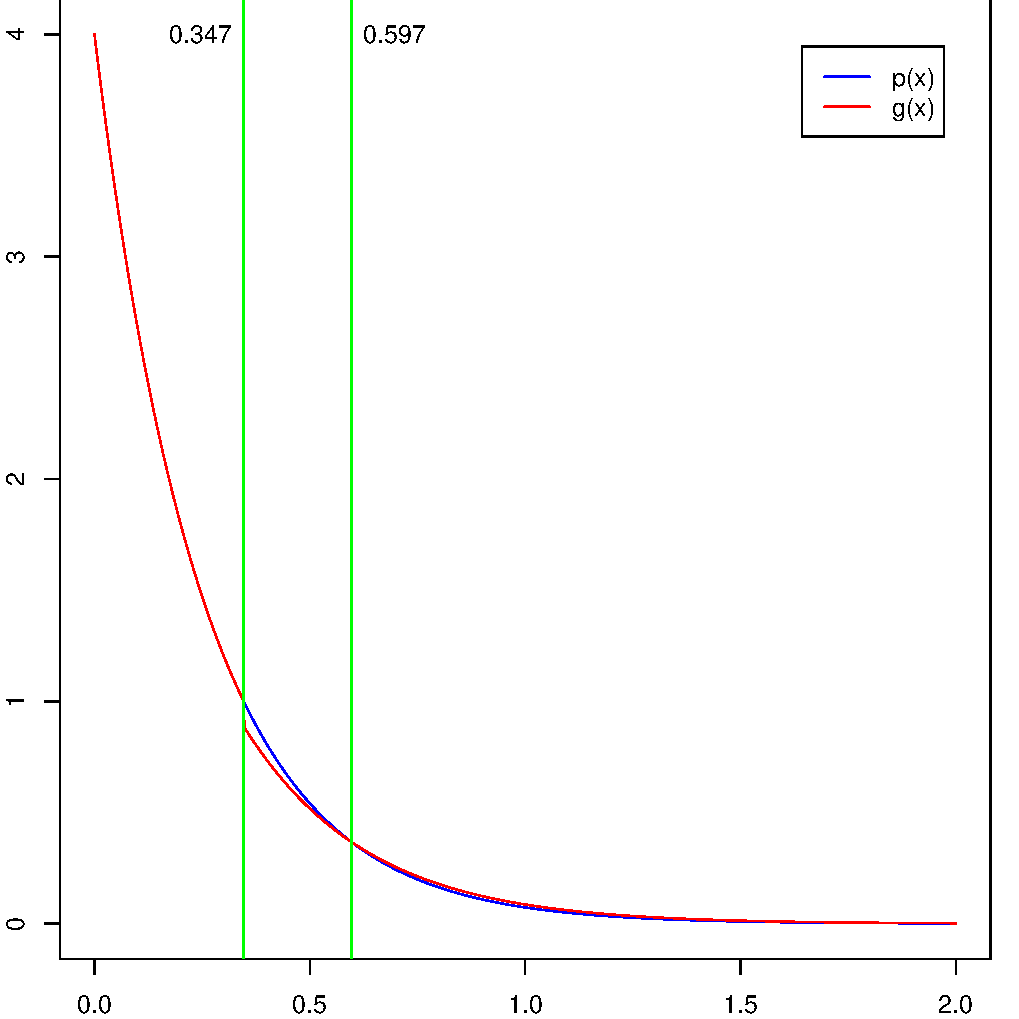
\includegraphics[width=0.7\linewidth]{plot}}
\caption{Распределение $g(x), p(x)$}
\label{ris:plot}
\end{figure}


% A

\subsection{Область $A=[0, x_1)$}

Область $A$ не отличается от исходного показательного распределения. Ее моделирование не представляет никакой сложности. Площадь данного участка выражается через функцию экспоненциального распределения вероятности и равна $S_A=\beta$.

% B

\subsection{Область $B=[x_1, x_2)$}

В области $B$ применим метод мажорант. Моделирование проходит по следующему алгоритму~\cite{MonErm}:
\begin{algo}[Метод мажорант]
Пусть 
$$D_S=\frac{\int_S p(x) dx}{\int_S g(x) dx},$$
где $g(x)$ --- моделируемая плотность, $p(x)$ --- некоторая другая плотность, такая, что $\forall x \in S \ p(x) \ge g(x)$. Тогда:
\begin{enumerate}
\item получим реализацию $\xi \sim \frac{p(X)}{|D|}$;
\item получим реализацию $\eta_{s+1} ~U(0, p(\xi))$;
\item если $\eta_{s+1} > g(\xi)$, переходим к пункту 1; иначе $\xi$ --- искомая случайная величина, $\xi \sim g(x)$.
\end{enumerate}
Эффективность метода равна $\frac{1}{|D_B|}$.
\end{algo}

Отношение интегралов функций в данной области успешно выражается при помощи формулы~\eqref{eq:gint} и следующих замечаний:
\begin{equation}\label{eq:ex1x2}
e^{-\alpha x_1}=1-\beta, e^{-\alpha x_2}=\frac{1-\beta}{e}.
\end{equation}

С учетом этого площадь $g(x), x \in B$ и отношение площадей $\frac{p(x)}{g(x)}, x \in B$ принимает вид: 
$$
S_B=\int_B g(x)dx=\frac{e-1}{e}(1-\beta-b_nx_2+\frac{b_n}{\alpha})+b_n(x_1-\frac{x_2}{e});
$$
$$
D_B=\frac{\int_B p(x)dx}{\int_B g(x) dx}= \frac{1-\beta}{1-\beta+b_n(\frac{1}{\alpha}+\frac{e}{e-1}(x_1-x_2))}.
$$

Результат моделирования распределения в виде гистограммы с наложенными функциями $g(x), p(x)$ представлен на рисунке~\ref{ris:sectionB}. 

\begin{figure}[h]
\center{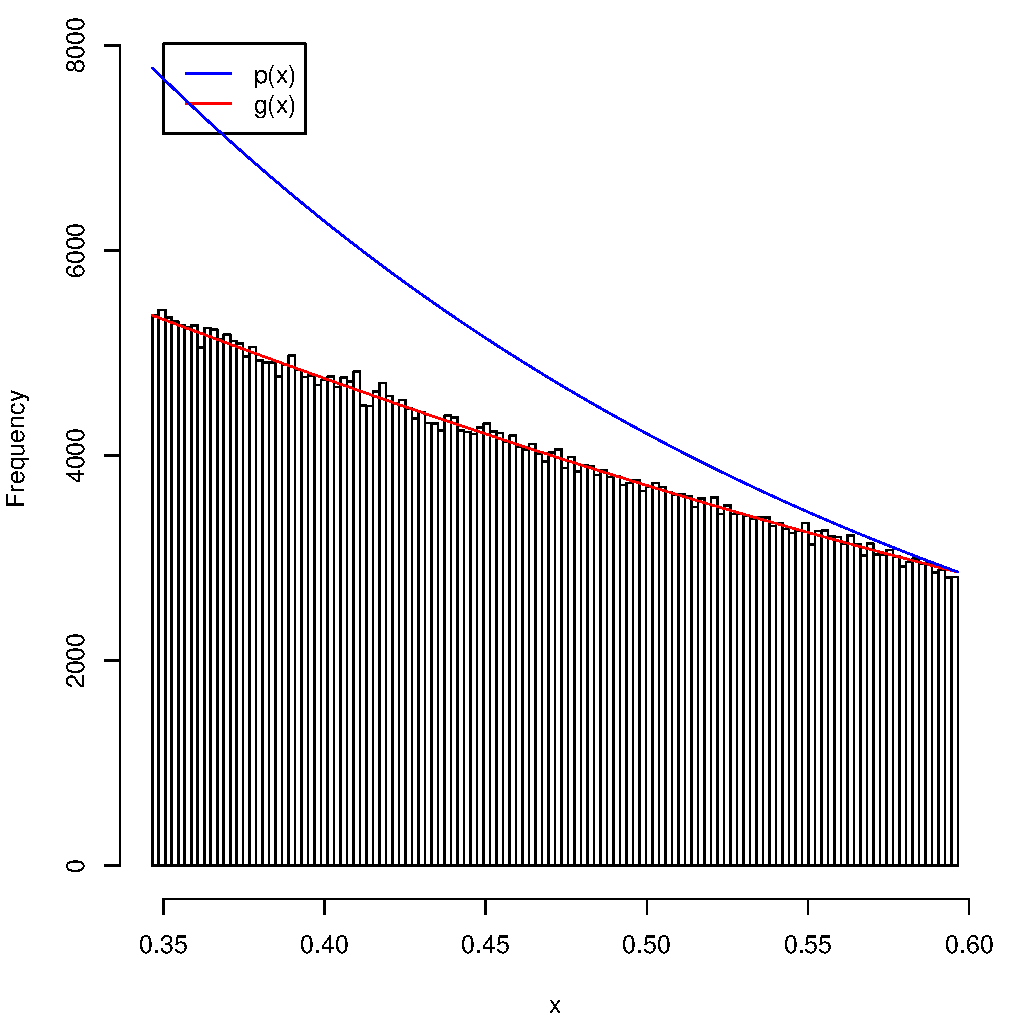
\includegraphics[width=0.7\linewidth]{sectionB}}
\caption{Распределение $g(x), p(x)$ при $x \in B$}
\label{ris:sectionB}
\end{figure}


% C

\subsection{Область $C=[x_2, \infty)$}

В области $C$ используем метод композиции~\cite{MonErm}. 

\begin{algo}[Метод композиции]\label{alg:comp}
Пусть искомая плотность $g(x)$ представлена суммой плотностей $p_i(x)$ с некоторыми неотрицательными весами $a_i$:
\begin{equation}\label{eq:comp_common}
g(x)=\sum\limits_{i=1}^M a_ip_i(x).
\end{equation}

Тогда метод выражается следующим алгоритмом:
\begin{enumerate}
\item получаем реализацию $\xi \sim U(0, \sum_i a_i)$;
\item выбираем индекс $s=\arg\max(a_i:a_i<\xi);$
\item искомая случайная величина --- $\eta \sim p_s(x)$.
\end{enumerate}
\end{algo}


Представим функцию в виде:
$$
g(x)=p(x)(1+b_nh(x))=\alpha e^{-\alpha x} + \frac{b_n(x-x_2)}{1-\beta}\alpha e^{-\alpha x}=p(x)+p_1(x).
$$

Заменим во второй части $y=x-x_2$:
$$
p_1(y)=\frac{b_ny}{1-\beta}\alpha e^{-\alpha (y+x_2)}=
\frac{b_n}{\alpha(1-\beta)}\alpha^2 ye^{-\alpha y}e^{-\alpha x_2}=
\frac{b_ne}{\alpha}\alpha^2 ye^{-\alpha y}.
$$

Теперь $p_1(y)$ выражается гамма-распределением с параметрами $shape=2, scale=\frac{1}{\alpha}$. Получаем форму~\eqref{eq:comp_common} с весами $a_1=1, a_2=\frac{b_ne}{\alpha}$ и распределениями 

$$
p_1(x)=p(x)=exp(x, \alpha),
$$ 
$$
p_2(x)=\gamma(x, 2, \frac{1}{\alpha})+x_2.
$$
Используя формулу~\eqref{eq:gint} и замечания~\eqref{eq:ex1x2}, получаем формулу для площади $g(x):x \in C$:
$$
\int_C g(x)dx=\frac{\alpha-\alpha\beta+b_n}{\alpha e}.
$$

Результат моделирования распределения в виде гистограммы с наложенными функциями $g(x), p(x)$ представлен на рисунке~\ref{ris:sectionC}. 

\begin{figure}[h]
\center{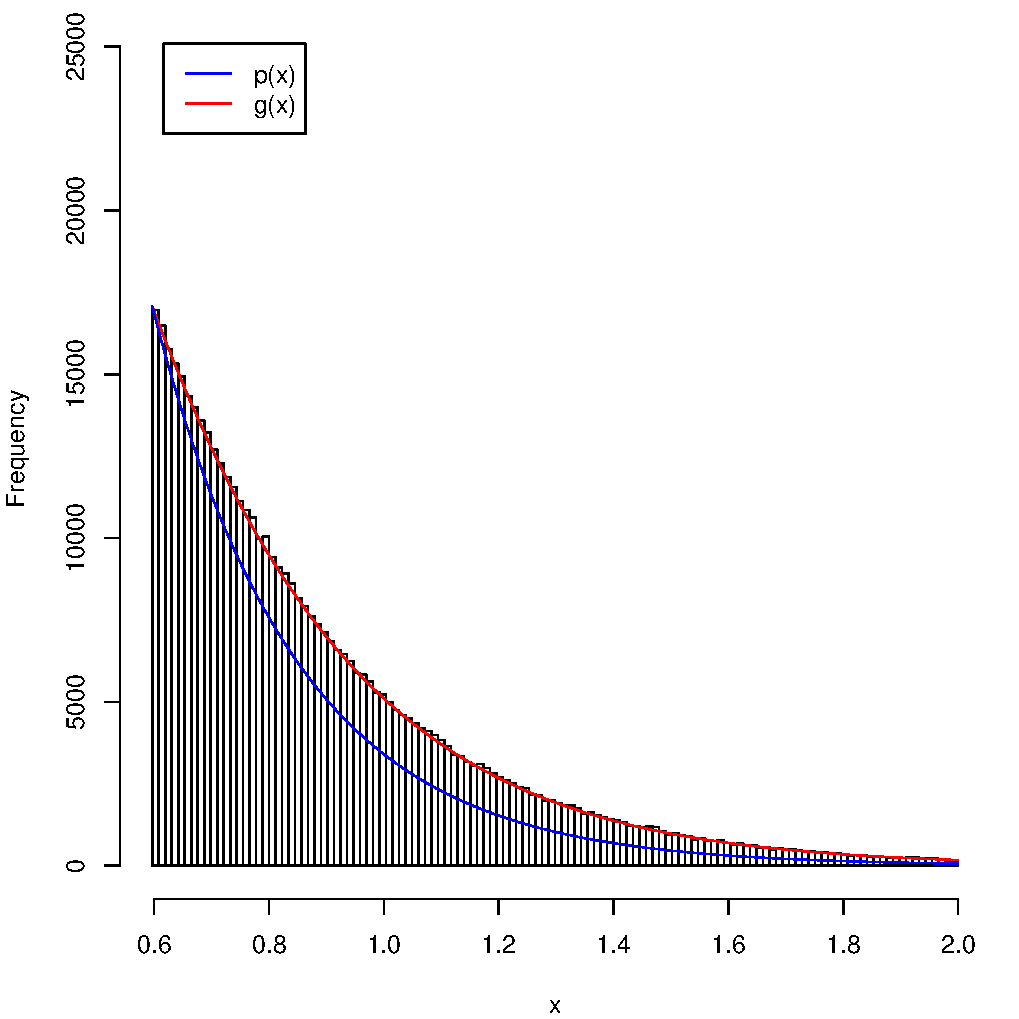
\includegraphics[width=0.7\linewidth]{sectionC}}
\caption{Распределение $g(x), p(x)$ при $x \in C$}
\label{ris:sectionC}
\end{figure}


% sum

\subsection{Моделирование общего распределения $g(x)$}

Моделирование проводится при помощи алгоритма~\ref{alg:comp}. В качестве весов берутся площади плотности $g(x)$ в соответствующих областях. Результат моделирования распределения в виде гистограммы с наложенными функциями $g(x), p(x)$ представлен на рисунке~\ref{ris:sectionAll}. 

\begin{figure}[h]
\center{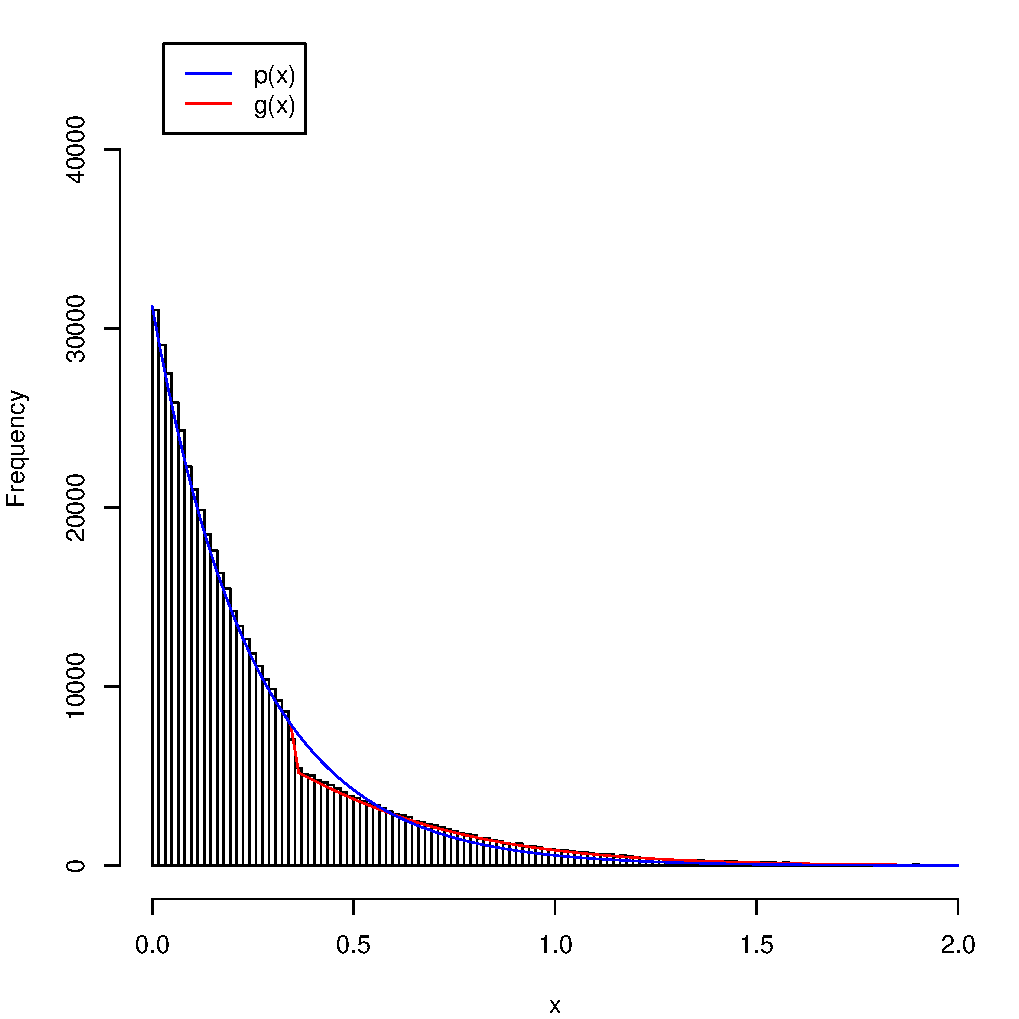
\includegraphics[width=0.7\linewidth]{sectionAll}}
\caption{Распределение $g(x), p(x)$}
\label{ris:sectionAll}
\end{figure}

% интервал

\subsection{Вычисление доверительного интервала}

Строим $k$ выборок по $n$ реализаций, $Y^{(k)}_n \sim g(x).$ Выберем $n$ достаточно небольшим. По~\eqref{eq:sv_sd} имеем оценку вероятности:
$$
\hat{\omega}_n=\frac{1}{k} \sum\limits_{i=1}^{k}
\chi \big(T(\hat{Q}^{(i)}_n)-T(P_0) > b_n\big)
\prod\limits_{j=1}^{n} \frac{1}{1+b_nh(Y_j^{(i)})};
$$
$$
U_n=\frac{1}{k} \sum\limits_{i=1}^{k}
\chi \big(T(\hat{Q}^{(1)}_n)-T(P) > b_n\big)
\prod\limits_{j=1}^{n} \frac{1}{(1+b_nh(Y_j^{(i)}))^2}.
$$

Дисперсия оценки вероятности $V=U_n-\hat\omega_n^2$.

Для демонстрации работы алгоритма были построены доверительные интервалы $\omega$ для следующих параметров: $\alpha=4, \beta=0.9, \gamma \in [0.8, 0.99] n=500, k=1000$ и $k=2000$. 

Выбор $\alpha$ обусловлен лишь ограничением на конечность дисперсии: $\alpha > 2.$ Выбор $\beta$ сделан исходя из стандартной практики в данной области, ее значение выбирают в зависимости от объема выборки в диапазоне от $0.8$ до $0.9$; $\gamma$ это уровень доверия вероятности $\omega$. Следует учесть, что при моделировании необходимо перестраивать плотность $g(x)$ каждый раз при изменении $\gamma$, так как от нее зависит $b_n$~\eqref{eq:bn}. Итоговые доверительные интервалы показаны на рисунках~\ref{ris:dover1} и ~\ref{ris:dover2}.

\begin{figure}[h]
\center{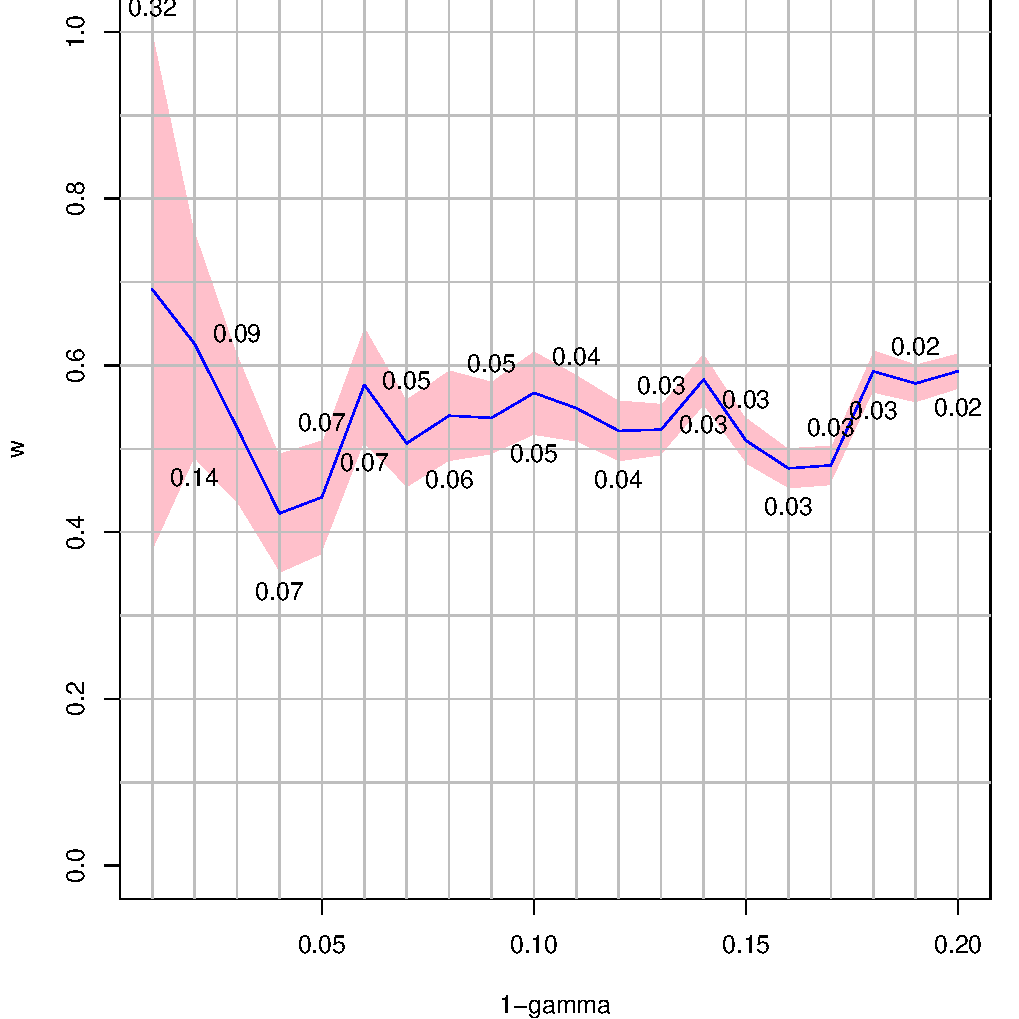
\includegraphics[width=0.6\linewidth]{dover1}}
\caption{Оценка $\omega$ и доверительный интервал при $k=1000$.}
\label{ris:dover1}
\end{figure}

\begin{figure}[h]
\center{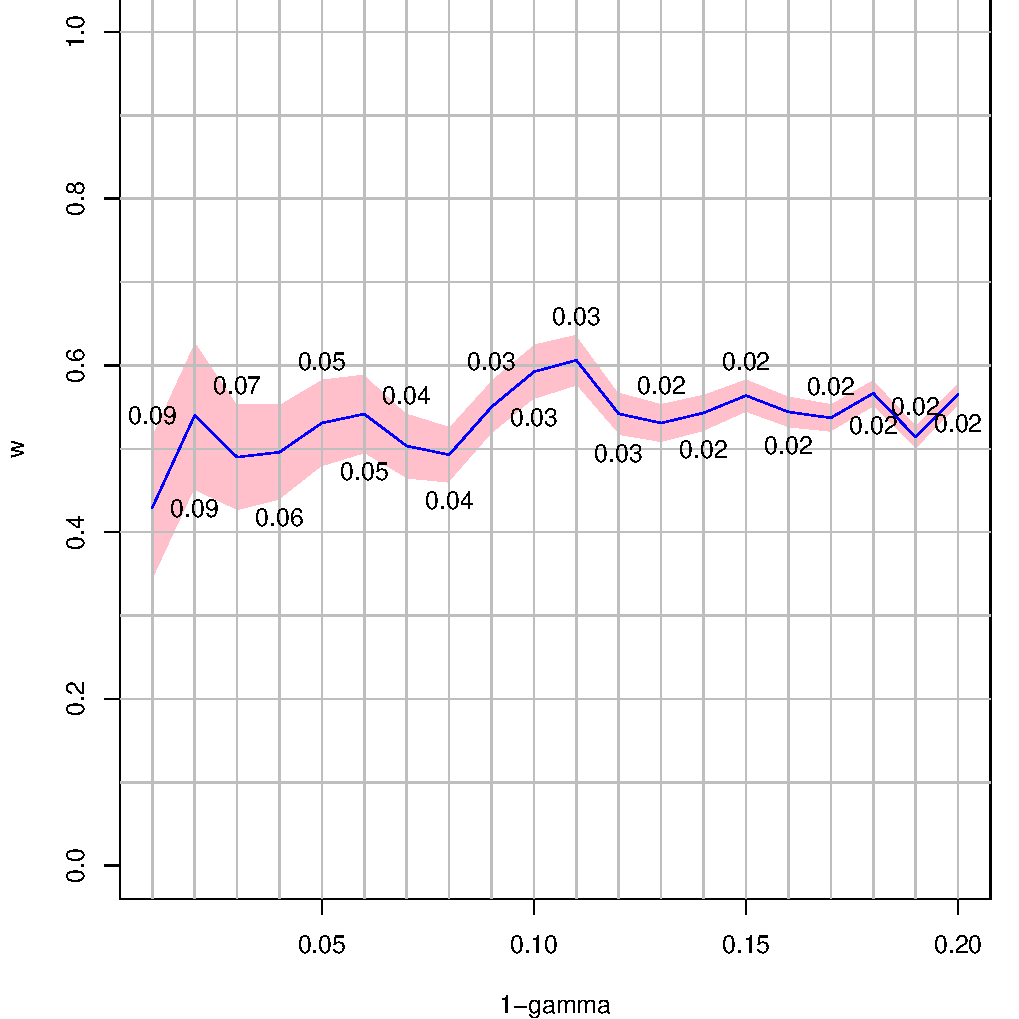
\includegraphics[width=0.6\linewidth]{dover2}}
\caption{Оценка $\omega$ и доверительный интервал при $k=2000$.}
\label{ris:dover2}
\end{figure}

% Заключение

\conclusion

В работе исследована задача построения доверительного интервала для вероятности уклонения параметра формы (\textit{shape}), полученного при помощи оценки Хилла. Задача решалась на основе асимптотической эффективности метода существенной выборки для $b_n>0$.

В дальнейшем планируется рассмотреть способы оценки полученных результатов. Необходимо исследовать эффективность метода по сравнению с обычным доверительным оцениванием. Также планируется рассмотреть построение доверительных интервалов других оценок параметров асимптотических распределений. 



\bibliographystyle{gost2008}
\bibliography{diploma3}

\end{document}